\documentclass[onecolumn]{elsart3p}
\usepackage{natbib}
\usepackage{amsmath}
\usepackage{amsfonts}
\usepackage{amssymb}
\usepackage{graphicx}%
\usepackage{subfigure} % Written by Steven Douglas Cochran
\bibliographystyle{plain}
%%%%%%%%%%%%%%%%%%% epsfig inputd by souto
%%%%%%%%%%%%%%%%%%%%%%%%
\journal{SPHERIC 2013}
\setlength{\textheight}{25cm}
\begin{document}
%\newpage
%\tableofcontents
%\newpage
%%%%%%%%%%%%%%%%%%%%%%%%%%%%%%%%%%%%%%%%%%%%%%%%%%%%

\begin{frontmatter}

$$\;$$
\vspace{-7cm}
\title{Applications and improvements of the PFEM (particles + finite elements) methodology to free surface flows.}
%
%
\author{J.M. Gimenez},
\address{CIMEC,
Universidad Nacional del Litoral (UNL). Santa F\'{e}, Argentina.}
%
\author{P. Gal\'{a}n del Sastre,}
\author{L.M. Gonz\'{a}lez\corauthref{cor}}
\corauth[cor]{Corresponding author.} \ead{leo.gonzalez@upm.es}
\address{Technical University of Madrid (UPM). 28040 Madrid, Spain.}
% \address{Naval Architecture Department (ETSIN),
% Technical University of Madrid (UPM). 28040 Madrid, Spain.}%
\vspace{-0.8cm}
\begin{abstract}

This work presents an alternative technology that combines a Lagrangian particle evolution and the finite element method. Both methodologies are designed to obtain several advantages:

\begin{itemize}
  \item Longer time steps compared to the pure Eulerian methodology giving a fast and stable temporal scheme for long time simulations.
  \item The presence of a fixed mesh that supports a finite element base apport high accuracy to this method.
  \item A semi-Lagrangian scheme where the convective term is not explicitly present is used, where the flow information is interpolated between the mesh nodes and the particle positions giving a double perspective.
  \item Boundary conditions are implemented in the mesh nodes similarly to finite element methodology.
\end{itemize}

Particle-Finite element method (PFEM)\cite{onate04} has been widely used as a useful numerical technique in different applications. In the first versions of the PFEM, mesh nodes moved like particle transporting the fluid properties, and re-meshing was necessary. An improved version of this method, known as PFEM-2 was developed, see \cite{idelsohn_etal_13}, where the mesh remains fixed and particles transport information following the fluid streamlines and interact with the mesh nodes via interpolation. Based on this second version, an efficient numerical algorithm is presented and tested for a wide number of problems involving free surface flows with different aspect ratio between the densities and viscosities of the fluids involved. Most of the problems selected have either reference numerical solutions or experimental results in order to compare the accuracy given by PFEM-2. This method has been used in typical free surface problems as: sloshing, standing waves, Rayleigh-Taylor instabilities and violent dam-break problems. In Figure \ref{foto} 
two different results are shown, first a typical and well studied flow around a circular cylinder is solved to confirm that this method is also valid when there is just one fluid involved in the computation. Second, a Rayleigh-Taylor instability with a low density ratio is studied, the evolution of the interface between both fluids was successfully compared with other numerical methodologies. The treatment of the interface has been simulated using a well known technique as Level-Set method \cite{sussman1994}, but the implementation of this methodology has been highly improved adding different levels of completeness to the original enrichment idea \cite{Coppola} in order to improve the free-surface computation.
\end{abstract}

\end{frontmatter}

\vspace{-0.5cm}

\begin{figure}[ht]
\centering
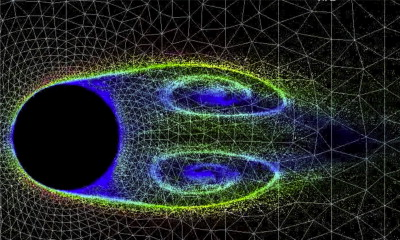
\includegraphics[height=4.5cm]{fixedMeshAndParticles.jpg}
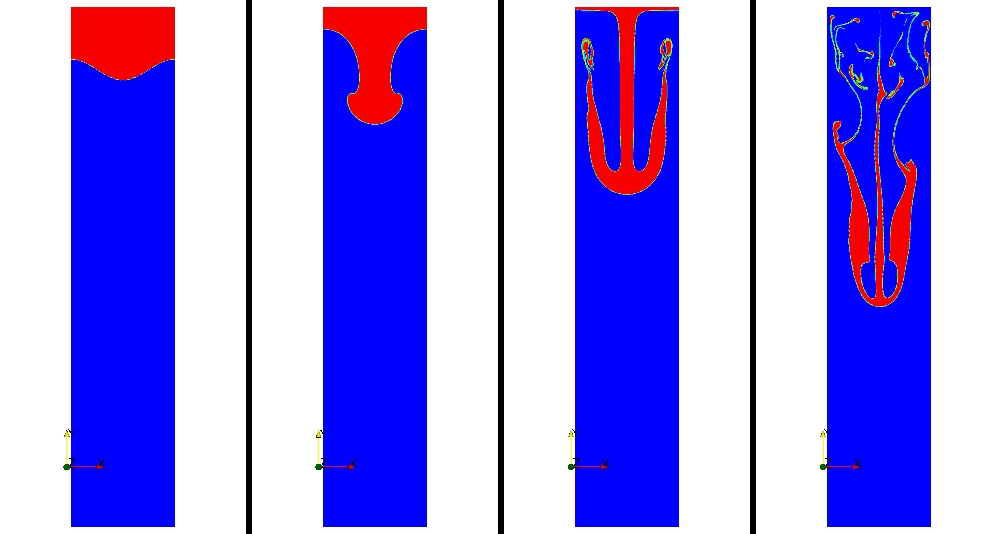
\includegraphics[height=4.5cm]{sequence_rayleigh.jpg}
%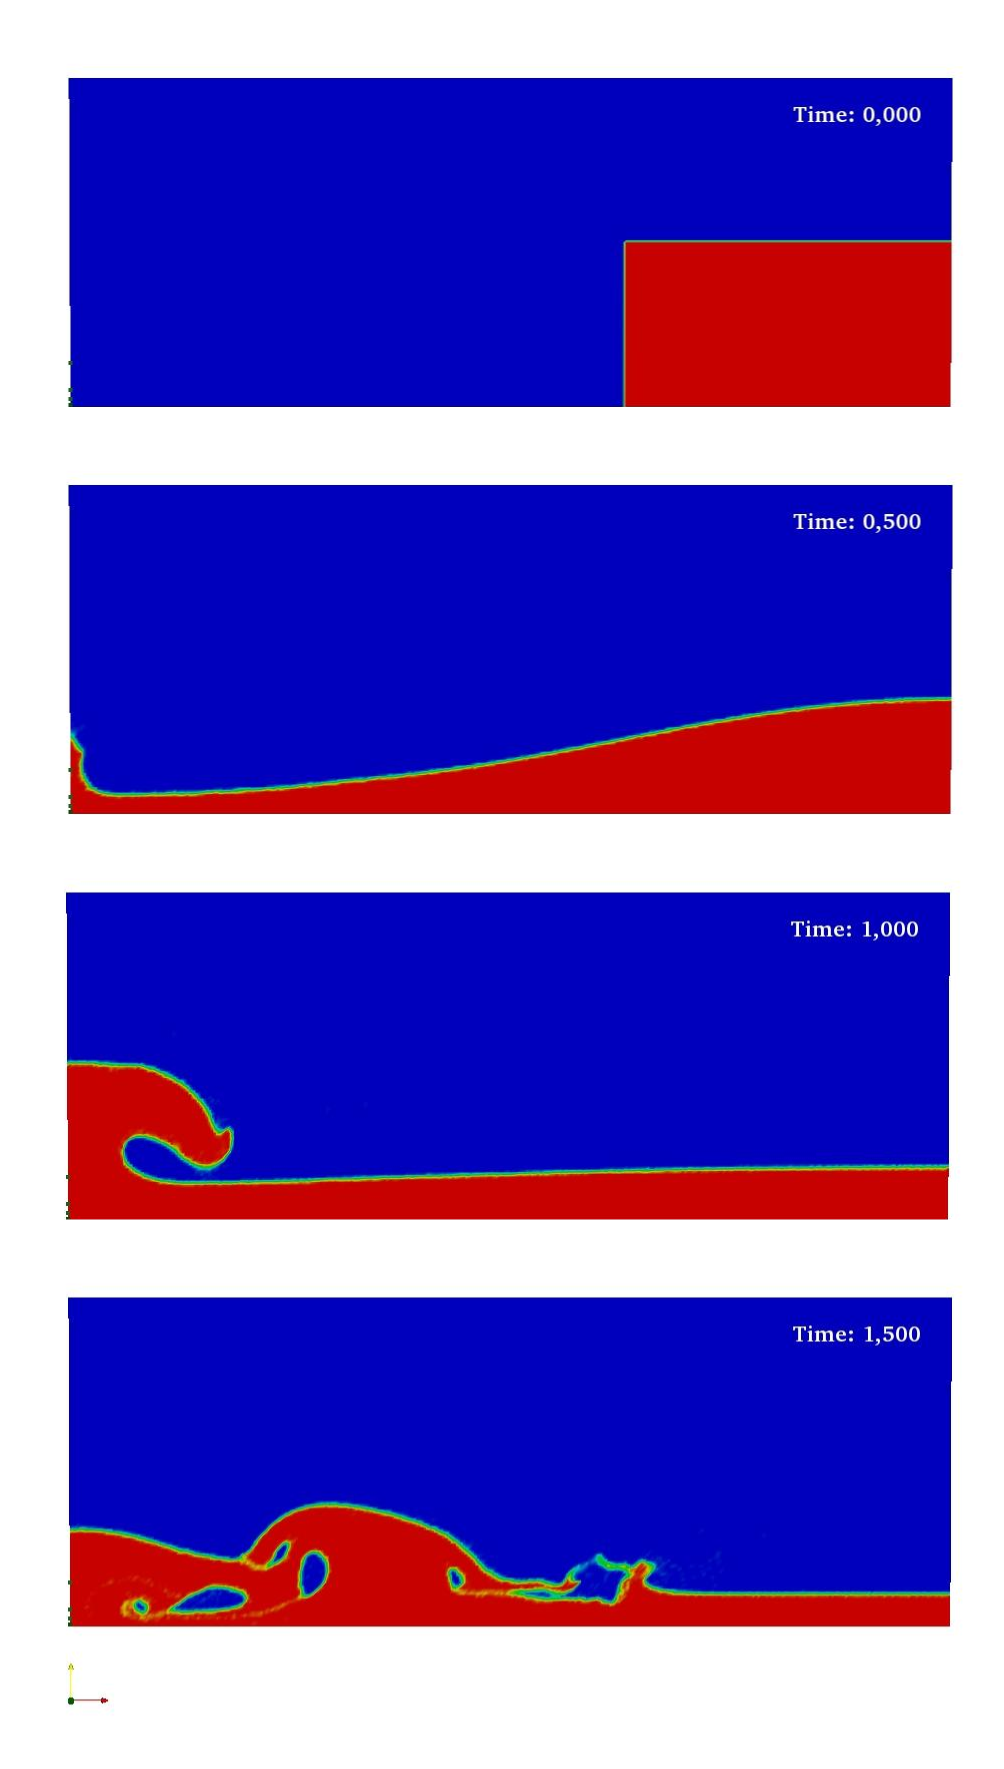
\includegraphics[height=5cm]{sequence_dam_break.jpg}
\caption{Left: Graphical description of the method PFEM-2. It contains a fixed mesh and a cloud of particles\cite{idelsohn_etal_13}.
%Screenshots for the dam-break case at times T=0, 0.5, 1 and 1.5 [s] respectly. Pressure values on left wall and heights measurement shows a good agreement with experimental results." (L. Lobovsky, E. Botia-Vera, F. Castellana, J. Mas-Soler and A. Souto-Iglesias , \emph{Experimental investigation of dynamic pressure loads during dam break}, Journal of Fluids and Structures, submitted, 2013.)
Right: Screenshots for the evolution of the Rayleigh-Taylor instability. Sequence of the free surface position shows the development of the mushroom-like structure, according to reference results\cite{Strubelj2011}.}
\label{foto}
\end{figure}


%%%%%%%%%%%%%%%%%%%%%%%%%%%%%%%%%%%%%%%%%%%%%%%%%%%%%%
%%%%%%%%%%%%%%%%%%%%%%%%%%%%%%%%%%%%%%%%%%%%%%%%%%%%%%
\bibliography{bib}
\end{document}
